\section{Внутренние форматы хранения данных}
\setcounter{figure}{0}

% The 3-Clause BSD License

В данной работе используется комбинация из различных структур данных, 
объединённых в единую систему.
Полная схема структур и их связей представленна на рис. \ref{overall_data_structure} 

\begin{figure}[hpt!]
    \centering
    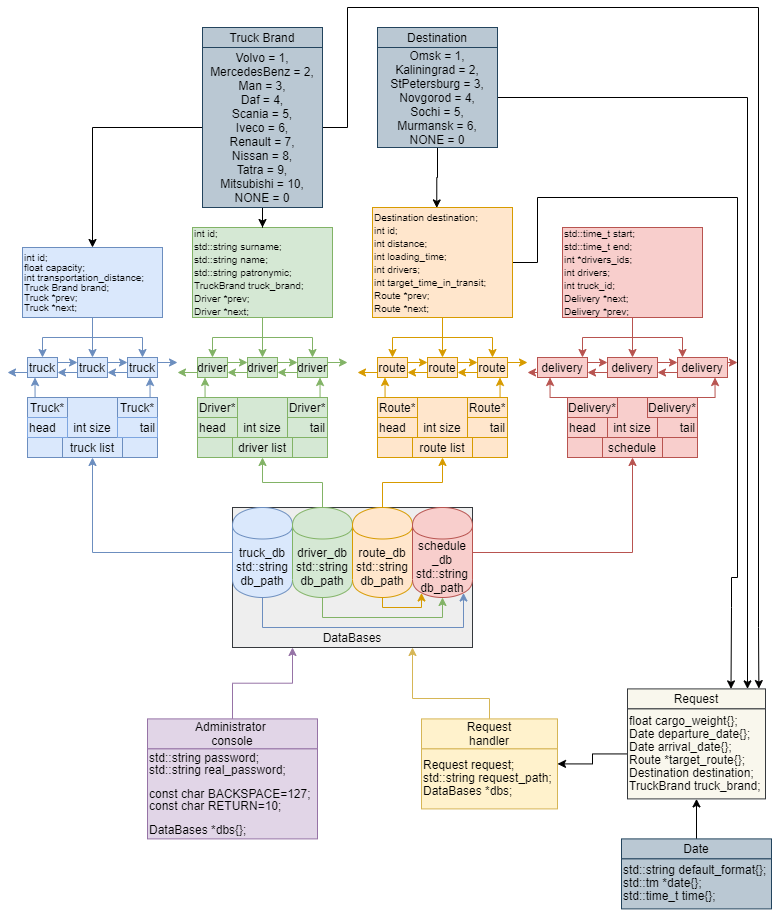
\includegraphics[width=1\linewidth]{photo/overall_data_structure}
    \caption{Обзорная диаграмма структур данных программы}
    \label{overall_data_structure}
\end{figure}

\newpage

\subsection{Структура данных двусвязный список}

В работе предпологается использование структуры данных "список".
Список --- структура данных, состоящая из элементов, 
содержащих помимо собственных данных ссылки на 
следующий и/или предыдущий элемент списка \cite{list_defenition}.

Для работы был вабран вариант с двунаправленым списком, 
где каждый узел имеет указатель на следующий и на предыдущий элементы.
Схема двунаправленного списка показана на рис. \ref{list_schema}.

\begin{figure}[hpt!]
    \centering
    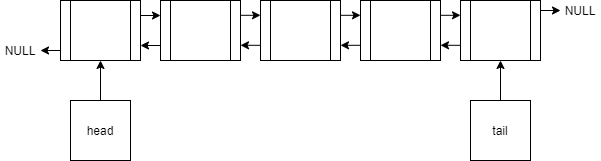
\includegraphics[width=1\linewidth]{photo/list_schema}
    \caption{Схема структуры данных двусвязный список}
    \label{list_schema}
\end{figure}

\subsection{TruckBrand}

Структурой данных \textbf{перечисление} представленны марки грузовиков.
Здесь содержаться все возможные значения марок грузовиков транспортной компании. 

Схема представлена на рис. \ref{truck_brand}

\begin{figure}[hpt!]
    \centering
    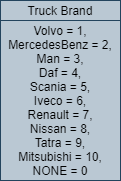
\includegraphics[width=0.2\linewidth]{photo/truck_brand}
    \caption{Перечисление TruckBrand}
    \label{truck_brand}
\end{figure}

\subsection{Destination}


Возможные маршруты поставки содержаться в структуре данных  \textbf{перечисление}.
Здесь содержаться все возможные значения маршрутов транспортной компании. 

Схема представлена на рис. \ref{destination}

\begin{figure}[hpt!]
    \centering
    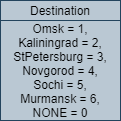
\includegraphics[width=0.4\linewidth]{photo/destination}
    \caption{destination}
    \label{destination}
\end{figure}

\subsection{Truck}

Представление грузовика в памяти программы выполнено в виде структуры Truck со следующими полями:

\begin{itemize}
    \item int id; -- идентификатор грузовика
    \item float capacity; -- максимальна масса груза
    \item int transportation\_distance; -- дальность перевозки
    \item TruckBrand brand; -- марка
    \item Truck *prev; -- указатель на предыдущий элемент
    \item Truck *next; -- указатель  на следующий элемент
\end{itemize}

Схема на рис. \ref{truck}.

\begin{figure}[H]
    \centering
    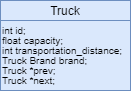
\includegraphics[width=0.4\linewidth]{photo/truck}
    \caption{truck}
    \label{truck}
\end{figure}

\subsection{TruckList}

Для управления списком грузовиков используется структура TruckList со следующими полями:

\begin{itemize}
    \item Truck *head; -- указатель на первый элемент списка
    \item Truck *tail; -- указатель на последний элемент списка
    \item int size; -- количество элементов в списке
\end{itemize}

Структура так же содержит методы для управления списком.

Схема на рис. \ref{truck_list}.

\begin{figure}[hpt!]
    \centering
    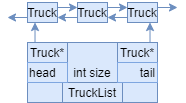
\includegraphics[width=0.4\linewidth]{photo/truck_list}
    \caption{truck\_list}
    \label{truck_list}
\end{figure}

\subsection{TruckDataBase}

Для управления базой данных грузовиков, 
её загрузки и обновления, 
используется структура TruckDataBase со следующими полями: 

\begin{itemize}
    \item TruckList list{}; -- список
    \item std::string db\_path{}; -- путь к файлу с базой данных
    \item ScheduleDataBase *schedule{}; -- указатель на расписание
\end{itemize}

Структура так же содержит методы для управления базой данных.

Схема на рис. \ref{truck_db}.

\begin{figure}[H]
    \centering
    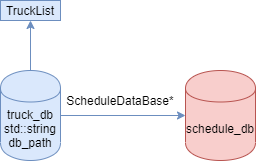
\includegraphics[width=0.4\linewidth]{photo/truck_db}
    \caption{truck\_db}
    \label{truck_db}
\end{figure}

\subsection{Route}

Представление маршрута в памяти программы выполнено в виде структуры Route со следующими полями:

\begin{itemize}
    \item Destination destination; -- точка прибытия
    \item int id; -- идентификатор маршрута
    \item int distance; -- дальность перевозки (в одну сторону)
    \item int loading\_time; -- время погрузки/разгрузки
    \item int drivers; -- количество водителей
    \item int target\_time\_in\_transit; -- время в пути (в одну сторону)
    \item Route *prev; -- указатель на предыдущий элемент
    \item Route *next; -- указатель на следующий элемент
\end{itemize}

Схема на рис. \ref{route}.

\begin{figure}[hpt!]
    \centering
    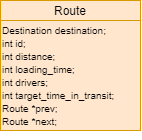
\includegraphics[width=0.4\linewidth]{photo/route}
    \caption{route}
    \label{route}
\end{figure}

\subsection{RouteList}

Для управления списком маршрутов используется структура RouteList со следующими полями:

\begin{itemize}
    \item Route *head; -- указатель на первый элемент списка
    \item Route *tail; -- указатель на последний элемент списка
    \item int size; -- количество элементов в списке
\end{itemize}

Структура так же содержит методы для управления списком.

Схема на рис. \ref{route_list}.

\begin{figure}[hpt!]
    \centering
    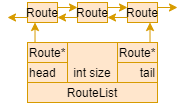
\includegraphics[width=0.4\linewidth]{photo/route_list}
    \caption{routelist}
    \label{route_list}
\end{figure}

\subsection{RouteDataBase}

Для управления базой данных маршрутов, 
её загрузки и обновления, 
используется структура RouteDataBase со следующими полями: 

\begin{itemize}
    \item RouteList list{}; -- список
    \item std::string db\_path{}; -- путь к файлу с базой данных
\end{itemize}

Структура так же содержит методы для управления базой данных.

Схема на рис. \ref{route_db}.

\begin{figure}[hpt!]
    \centering
    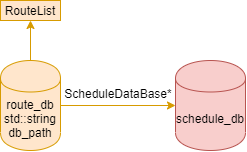
\includegraphics[width=0.4\linewidth]{photo/route_db}
    \caption{routedb}
    \label{route_db}
\end{figure}

\subsection{Driver}

Представление водителя в памяти программы выполнено в виде структуры Driver со следующими полями:

\begin{itemize}
    \item int id; -- идентификатор
    \item std::string surname; -- фамилия 
    \item std::string name; -- имя
    \item std::string patronymic; -- отчество
    \item TruckBrand truck\_brand; -- марка грузовика
    \item Driver *prev; -- указатель на предыдущий элемент
    \item Driver *next; -- указатель на следующий элемент
\end{itemize}

Схема на рис. \ref{driver}.

\begin{figure}[hpt!]
    \centering
    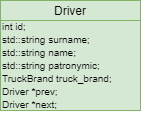
\includegraphics[width=0.4\linewidth]{photo/driver}
    \caption{driver}
    \label{driver}
\end{figure}

\subsection{DriverList}

Для управления списком водителей используется структура DriverList со следующими полями:

\begin{itemize}
    \item Driver *head; -- указатель на первый элемент списка
    \item Driver *tail; -- указатель на последний элемент списка
    \item int size; -- количество элементов в списке
\end{itemize}

Структура так же содержит методы для управления списком.

Схема на рис. \ref{driver_list}.

\begin{figure}[H]
    \centering
    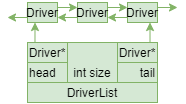
\includegraphics[width=0.4\linewidth]{photo/driver_list}
    \caption{driverlist}
    \label{driver_list}
\end{figure}

\subsection{DriverDataBase}

Для управления базой данных водителей, 
её загрузки и обновления, 
используется структура DriverDataBase со следующими полями: 

\begin{itemize}
    \item DriverList list{}; -- список
    \item std::string db\_path{}; -- путь к файлу с базой данных
    \item ScheduleDataBase *schedule{}; -- указатель на расписание
\end{itemize}

Структура так же содержит методы для управления базой данных.

Схема на рис. \ref{driver_db}.

\begin{figure}[hpt!]
    \centering
    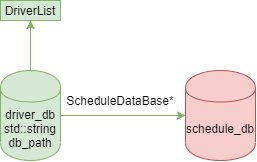
\includegraphics[width=0.4\linewidth]{photo/driver_db}
    \caption{driverdb}
    \label{driver_db}
\end{figure}

\subsection{Delivery}

Представление поставки в памяти программы выполнено в виде структуры Delivery со следующими полями:

\begin{itemize}
    \item std::time\_t start{}; -- время начала поставки
    \item std::time\_t end{}; -- время окончания поставки
    \item int *drivers\_ids{}; -- идентификаторы водителей
    \item int drivers{}; -- количество водителей
    \item int truck\_id{}; -- идентификатор грузовика
    \item Delivery *next{}; -- указатель на предыдущий элемент
    \item Delivery *prev{}; -- указатель на следующий элемент
\end{itemize}

Схема на рис. \ref{delivery}.

\begin{figure}[hpt!]
    \centering
    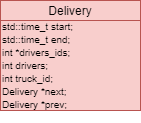
\includegraphics[width=0.4\linewidth]{photo/delivery}
    \caption{delivery}
    \label{delivery}
\end{figure}

\subsection{Schedule}

Для управления списком поставок используется структура Schedule со следующими полями:

\begin{itemize}
    \item Delivery *head; -- указатель на первый элемент списка
    \item Delivery *tail; -- указатель на последний элемент списка
    \item int size; -- количество элементов в списке
\end{itemize}

Структура так же содержит методы для управления списком.

Схема на рис. \ref{schedule}.

\begin{figure}[hpt!]
    \centering
    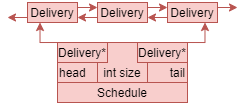
\includegraphics[width=0.4\linewidth]{photo/schedule}
    \caption{schedule}
    \label{schedule}
\end{figure}


\subsection{ScheduleDataBase}

Для управления базой данных поставок, 
её загрузки и обновления, 
используется структура DriverDataBase со следующими полями: 

\begin{itemize}
    \item Schedule list{}; -- список
    \item std::string db\_path{}; -- путь к файлу с базой данных
\end{itemize}

Структура так же содержит методы для управления базой данных.

Схема на рис. \ref{schedule_db}.

\begin{figure}[hpt!]
    \centering
    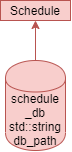
\includegraphics[width=0.2\linewidth]{photo/schedule_db}
    \caption{scheduledb}
    \label{schedule_db}
\end{figure}

\subsection{DataBases}

Объединяет все базы данных структура DataBases со следующими полями: 

\begin{itemize}
    \item ScheduleDataBase schedule\_db; -- база данных с расписанием
    \item TruckDataBase truck\_db; -- база данных с грузовиками
    \item DriverDataBase driver\_db; -- база данных с водителями
    \item RouteDataBase route\_db; -- база данных с маршрутами
\end{itemize}

Схема на рис. \ref{dbs}.

\begin{figure}[hpt!]
    \centering
    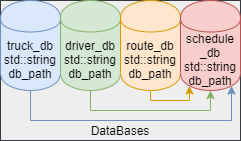
\includegraphics[width=0.4\linewidth]{photo/dbs}
    \caption{dbs}
    \label{dbs}
\end{figure}

\subsection{AdministratorConsole}

Консоль администратора представлена структурой AdministratorConsole со следующими полями: 

\begin{itemize}
    \item std::string password; -- пароль, вводимый пользователем
    \item std::string real\_password; -- заданный пароль (его хэш)
    \item const char BACKSPACE=127; -- ascii код символа backspace
    \item const char RETURN=10; -- ascii код символа return
    \item DataBases *dbs{}; -- указатель на базы данных
\end{itemize}

Структура так же содержит методы для управления базами данных.

Схема на рис. \ref{administrator_console}.

\begin{figure}[hpt!]
    \centering
    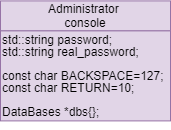
\includegraphics[width=0.4\linewidth]{photo/administrator_console}
    \caption{administratorconsole}
    \label{administrator_console}
\end{figure}

\subsection{Date}

Для управления датой и временем используется структура Date со следующими полями: 

\begin{itemize}
    \item std::string default\_format{}; -- формат преобразования строки по умолчанию
    \item std::tm *date{}; -- структура для хранения времени. необходима для получения форматированный строки со временем.
    \item std::time\_t time{}; -- время в секундах начиная с 1 янв 1970 г., необходимо для сравнительных и вычислительный действий в программе.
\end{itemize}

Схема на рис. \ref{date}.

\begin{figure}[hpt!]
    \centering
    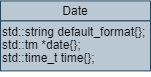
\includegraphics[width=0.4\linewidth]{photo/date}
    \caption{date}
    \label{date}
\end{figure}

\subsection{Request}

Запрос на поставку представлен в виде структуры Request со следующими полями: 

\begin{itemize}
    \item float cargo\_weight{}; -- масса груза
    \item Date departure\_date{}; -- дата отправки
    \item Date arrival\_date{}; -- дата прибытия (заполняется программой)
    \item Route *target\_route{}; -- маршрут (заполняется программой)
    \item Destination destination; -- точка прибытия
    \item TruckBrand truck\_brand; -- марка грузовика
\end{itemize}

Схема на рис. \ref{request}.

\begin{figure}[hpt!]
    \centering
    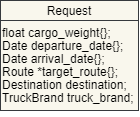
\includegraphics[width=0.4\linewidth]{photo/request}
    \caption{request}
    \label{request}
\end{figure}

\subsection{RequestHandler}

Для обработки запроса на поставку используется структура RequestHandler со следующими полями: 

\begin{itemize}
    \item Request request; -- запрос
    \item std::string request\_path; -- путь к файлу с запросом
    \item DataBases *dbs; -- указатель на базы данных
\end{itemize}

Схема на рис. \ref{request_handler}.

\begin{figure}[hpt!]
    \centering
    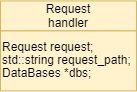
\includegraphics[width=0.4\linewidth]{photo/request_handler}
    \caption{requesthandler}
    \label{request_handler}
\end{figure}
